\chapter{Cálculos de subneteo}

\section{Fundamento}

Una dirección IPv4 contiene 32 bits. Un prefijo \code{/p} deja $h=32-p$ bits para identificar direcciones dentro de la subred. El tamaño total del bloque es:

\[
N_{\mathrm{total}} = 2^h = 2^{32-p}
\]

En una red tradicional suele enseñarse $N_{\mathrm{usable}}=2^h-2$ para descontar red y broadcast. AWS aplica una reserva distinta: las primeras cuatro direcciones y la última no pueden asignarse a una interfaz. Por tanto:

\[
N_{\mathrm{AWS}} = 2^{32-p}-5
\]

El número mínimo de bits de host para una demanda $H$ cumple:

\[
2^h-5 \geq H
\qquad\Longrightarrow\qquad
h=\left\lceil\log_2(H+5)\right\rceil,
\quad p=32-h
\]

Además de satisfacer la desigualdad, AWS impone \code{/28} como la subred IPv4 más pequeña permitida \cite{aws-subnet-sizing}. Todas las selecciones siguientes respetan ambos límites.

\section{Cálculo de Visitas}

El enunciado no fija cantidad, por lo que se declara $H=30$ visitantes concurrentes:

\[
h=\left\lceil\log_2(30+5)\right\rceil
=\left\lceil\log_2(35)\right\rceil
=\lceil5.13\rceil=6
\]

\[
p=32-6=26,\qquad
N_{\mathrm{total}}=2^6=64,\qquad
N_{\mathrm{AWS}}=64-5=59
\]

Se asigna \code{10.10.0.0/26}, máscara \code{255.255.255.192}. El tamaño de bloque en el último octeto es $256-192=64$. La red inicia en .0 y termina en .63. AWS reserva .0, .1, .2, .3 y .63; el rango asignable es .4--.62. La ocupación inicial prevista es $30/59=50.85\%$.

\section{Cálculo de Ventas}

Para $H=25$:

\[
h=\left\lceil\log_2(25+5)\right\rceil
=\left\lceil\log_2(30)\right\rceil=5,
\quad p=27
\]

El mínimo matemático es \code{/27}: $2^5-5=27$ direcciones asignables. Sin embargo, después de asignar una dirección a cada persona quedarían sólo dos. La holgura sería:

\[
\frac{27-25}{27}\times100=7.41\%
\]

Esta reserva es insuficiente si cada colaborador usa más de un dispositivo o si aparecen interfaces de servicios. Se selecciona operativamente \code{/26}:

\[
N_{\mathrm{AWS}}=2^6-5=59,qquad
\text{ocupación}=\frac{25}{59}\times100=42.37\%
\]

La subred es \code{10.10.0.64/26}. Su intervalo completo es .64--.127; AWS reserva .64--.67 y .127; el rango asignable es .68--.126. Esta decisión distingue el valor mínimo del valor recomendado y documenta el costo de la holgura.

\section{Cálculo de TI}

Para $H=15$:

\[
h=\left\lceil\log_2(15+5)\right\rceil
=\left\lceil\log_2(20)\right\rceil=5,
\qquad p=27
\]

Un \code{/28} tendría 16 direcciones totales y sólo 11 asignables en AWS, por lo que no cumple. Con \code{/27}, TI obtiene 27 asignables y 12 libres. Se asigna \code{10.10.0.128/27}, máscara \code{255.255.255.224} e incremento $256-224=32$. El bloque completo va de .128 a .159 y el rango asignable de .132 a .158.

\section{Cálculo de Data Center}

Para $H=5$:

\[
h=\left\lceil\log_2(5+5)\right\rceil
=\left\lceil\log_2(10)\right\rceil=4,
\qquad p=28
\]

La subred elegida es \code{10.10.0.160/28}. Contiene 16 direcciones y 11 asignables. Su máscara es \code{255.255.255.240} y el incremento es 16. AWS reserva .160--.163 y .175; los servidores pueden utilizar .164--.174. La capacidad libre es seis direcciones, equivalente al 54.55\% del espacio asignable.

\section{Cálculo de Administración}

El prototipo requiere un bastión y admite hasta tres componentes administrativos. Un bloque menor podría parecer suficiente matemáticamente. Sin embargo, AWS no permite subredes IPv4 más pequeñas que \code{/28}. Se asigna \code{10.10.0.176/28}. El intervalo completo es .176--.191, las direcciones reservadas son .176--.179 y .191, y el rango asignable es .180--.190.

\section{Resumen detallado}

\small
\begin{longtable}{p{2.4cm}p{2.8cm}p{2.3cm}p{2.9cm}p{2.5cm}}
\caption{Plan de direccionamiento IPv4}\label{tab:addressing}\\
\toprule
\textbf{Segmento} & \textbf{CIDR / máscara} & \textbf{Bloque completo} & \textbf{Reservas AWS} & \textbf{Asignables} \\
\midrule
\endfirsthead
\toprule
\textbf{Segmento} & \textbf{CIDR / máscara} & \textbf{Bloque completo} & \textbf{Reservas AWS} & \textbf{Asignables} \\
\midrule
\endhead
Visitas & \code{10.10.0.0/26} \newline 255.255.255.192 & .0--.63 & .0, .1, .2, .3, .63 & .4--.62 (59) \\
Ventas & \code{10.10.0.64/26} \newline 255.255.255.192 & .64--.127 & .64, .65, .66, .67, .127 & .68--.126 (59) \\
TI & \code{10.10.0.128/27} \newline 255.255.255.224 & .128--.159 & .128, .129, .130, .131, .159 & .132--.158 (27) \\
Data Center & \code{10.10.0.160/28} \newline 255.255.255.240 & .160--.175 & .160, .161, .162, .163, .175 & .164--.174 (11) \\
Administración & \code{10.10.0.176/28} \newline 255.255.255.240 & .176--.191 & .176, .177, .178, .179, .191 & .180--.190 (11) \\
Reserva & \code{10.10.0.192/26} \newline 255.255.255.192 & .192--.255 & No aplica hasta crear subred & 64 sin asignar \\
\bottomrule
\end{longtable}
\normalsize

\begin{figure}[H]
\centering
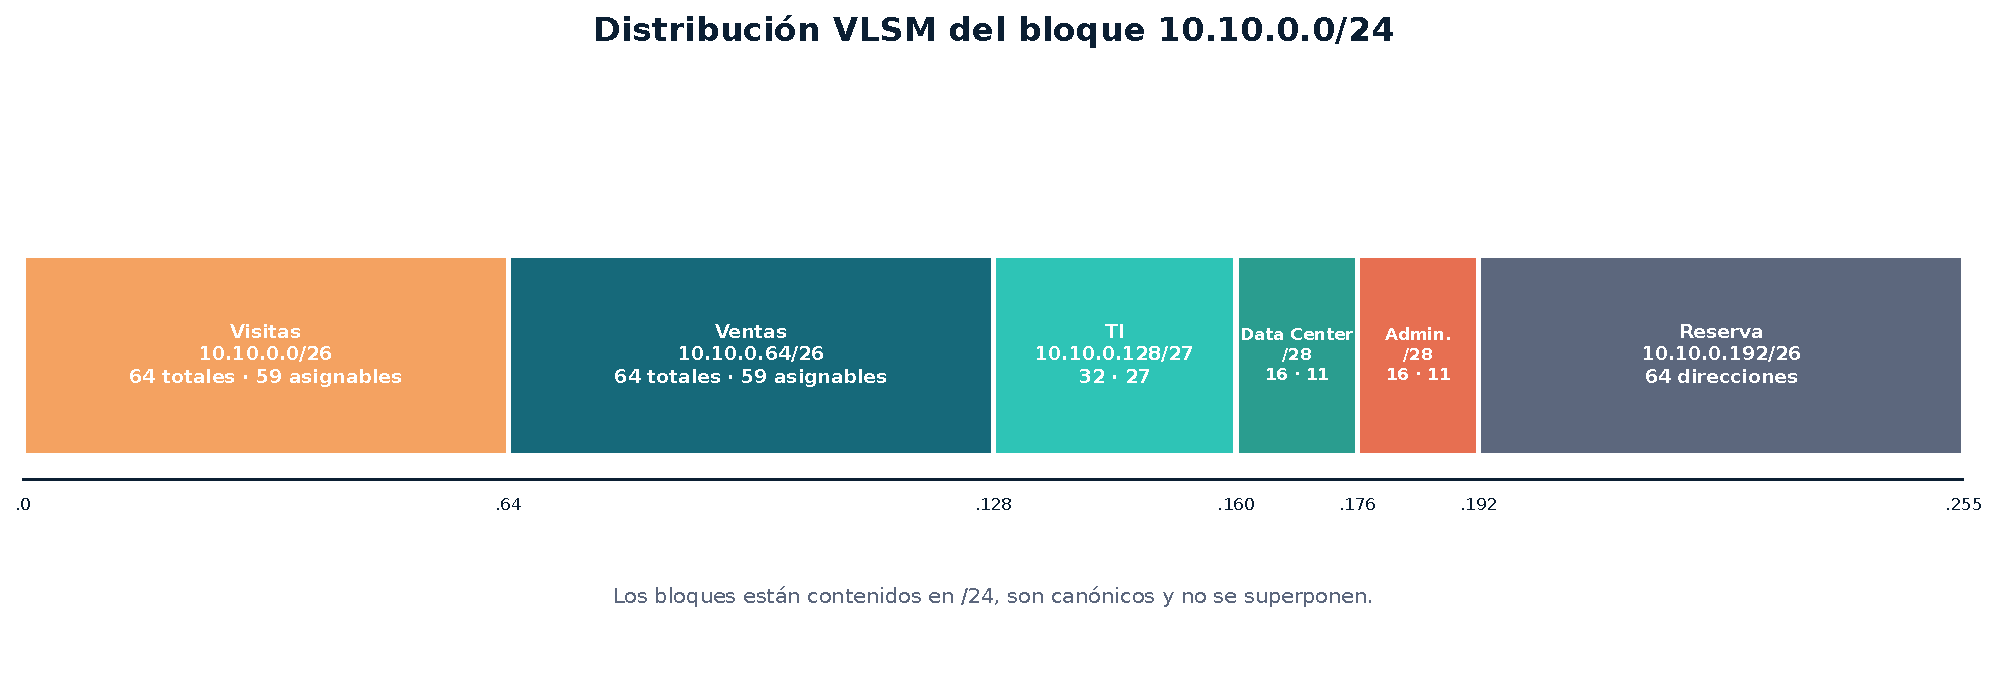
\includegraphics[width=\textwidth]{mapa-cidr.pdf}
\caption{Mapa proporcional del espacio de direcciones. Elaboración propia.}
\label{fig:cidr-map}
\end{figure}

\section{Demostración de contención y no solapamiento}

Los límites aparecen en múltiplos correctos de sus tamaños: 0 y 64 para bloques de 64; 128 para el bloque de 32; 160 y 176 para bloques de 16; y 192 para el bloque final de 64. Cada inicio coincide con el final anterior más uno. La suma es:

\[
64+64+32+16+16+64=256=2^8
\]

Por lo tanto, el plan cubre exactamente el \code{/24} sin huecos ni intersecciones. El script \path{scripts/validate-network.py} reproduce esta comprobación con la biblioteca estándar de Python. Su salida se conserva en \path{evidence/deployment/cidr-validation.txt}.
